%
		\subsection{Heating Mechanisms}\label{sec:heating}
%
		\paragraph{Ohmic Heating}
		In a spatially uniform electric field thas oscillates perpendicular to the electrodes harmonically, like it is the case in the bulk of a previously concerned ccrf discharge, electrons periodically gain and loose energy in the absence of collisions without any net energy gain~\cite{Schulze09}. This is due to the simmetrical de-/acceleration in the sheaths an main plasma volume over one rf cycle. Lets assume the electric field have no or a negligiable component parallel to the electrodes. Hence the mean absorbed power by the electrons in an oscillating electric field is
%
		\begin{align}
			\overline{P}\ix{ohm}=\omega\ix{rf}\int_{0}^{T\ix{rf}}\,j\ix{tot}(t)\cdot E(t)\diff t%
			\label{equ:meanpowerheat}\\[0.0cm]%
			m\ix{e}\frac{\diff v\ix{e}}{\diff t}=-eE(t)-m\ix{e}\nu\ix{n,e}v\ix{e}%
			\label{equ:heatingmotion}
		\end{align}
%
		The total charge current density $j\ix{tot}$ is the sum of displacement current from~\autoref{sec:displacementcurrent} and conduction current $en\ix{e,0}v\ix{e}\,$. Solving~\autoref{equ:heatingmotion} for the velocity, one yields and imagniary and real part due to the bulks impedance, like it was discussed earlier in~\autoref{sec:selfbias}. Substitution of this result~\cite{Schulze09} gives
%
		\begin{align}
			\overline{P}\ix{ohm}=\frac{|E\ix{0}|^{2}\Re(\sigma\ix{p})}{2}=%
			\frac{|j\ix{0}|^{2}}{2\Re(\sigma\ix{p})}\,,%
			\quad\quad%
			\sigma\ix{p}=\frac{n\ix{e}e^{2}}{m\ix{e}(\nu\ix{n,e}+\imag\omega\ix{p})}%
			\label{equ:ohmicheating}
		\end{align}
%
		This is, again, the total mean power dissipated into the electron species through accelration in a harmonically oscillating electric field and neutral gas friction. The property $\sigma\ix{p}$ is the plasma conductivity, hence yielding $j\ix{0}=\sigma\ix{p}E$. This shows that power from an spatially uniform, harmonically oscillating electric field can only be transferred via collisions. Elastic electron-neutrals collision transferred into a direction perpendicular to the field and is, hence, not lost during the reversal of $E(t)$. Therefore the electron species gains energy during the field oscillation. This mechanism is called \emph{ohmic heating} and takes place mainly in the plasma bulk.
%
		\paragraph{Stochastic Heating}
		Low-pressure, capacitively coupled rf plasma can primarily be stabilzed by collisionless heating in the sinusoidally  modulated discharge sheaths, like it was proposed earlier in~\autoref{sec:langmuirlaw} and the following. Most theoretical models assume a `hard wall' approximation (HWA), where the electrons are cosidered to collide elastically with the oscillating sheath edge. Heating power is then averaged by reverse and forward energy fluxes into and out of the sheath respectively. This gives an easy access to heating mechanisms of the proposed discharges.\\
		The heating mechanism in such low pressure plasma is of particular importance, because collisions are rare and sheath processes are key to the sustainabilty of the discharge (see e.g\@~\autoref{sec:bohmcriteria}). The afore-mentioned HWA uses the '\emph{fermi acceleration}' argument, which implies that the particles are heated or cooled due to the sheaths sinusoidal oscillation and a corresponding de-/accelration. This process, though relying on enough randomization in phase-space inside the bulk, sufficiently creates a net heating of the plasma~\cite{Gozadinos01b,Goedde88}. This is referred to as \emph{stochastic heating}.\\
		Here one will consider the sheaths electric field as constant, $E=U\ix{sb}/s\ix{0}$, the bulks expansion to be $l$  and the sheaths thickness $d$ being modulated cosinusoidal. The equation of motion for an electron in the sheath is taken from above, canceling out the part of ohmic neutral gas heating.
%
		\begin{align}
			d(t)\approx s\ix{0}\left(1+\frac{U\ix{rf}}{U\ix{sb}}\cos\left(\omega t\right)\right)%
			\label{equ:sheaththickness}
		\end{align}
%
		The~\autoref{equ:heatingmotion} is introduced as dimensionless with the corresponding parameters: $\alpha=m\ix{e}\omega^{2}s\ix{0}^{2}/(eU\ix{sb})$, $\beta=U\ix{rf}/U\ix{sb}$ and $\epsilon=s\ix{0}/l\,$. Integrating yields the velocity $\mu(\tau)$ of an electron as it moves through the sheath. The transit time $\tau$ is considered for one pass through the sheath of the particle. It can be used to calculate the change in velocity experienced by the electron on each bounce between this oscillating and a fixed wall --- this would be the lowest order \emph{fermi acceleration}. Assuming there are two distinct points in motion, where the particle enters (index $n$) and re-enters (index $n+1$) the sheath, this gives, using $\varphi\ix{n}$ the phase of the sheath, for the transit time and velocity~\cite{Goedde88}
%
		\begin{align}
			\tau\ix{n}\approx\frac{2\alpha(\mu\ix{n}-\beta%
				\cos\varphi\ix{n})}{1+\alpha\beta\cos\varphi\ix{n}}\,,%
			\quad\quad%
			\mu\ix{n+1}=-\mu+\frac{2(\mu\ix{n}-\beta\sin\varphi\ix{n})}{1+\alpha\beta\cos\varphi\ix{n}}%
			\label{equ:transitandvelocityheating}
		\end{align}
%
		In \emph{hamiltonian mappings}, those two variables are not canonically conjugate, hence insufficient for checking conservational properties. One has to keep that in mind when evaluating the HWA approximation. The change in velocity in one pass through the sheath becomes the impulse approximation of the \emph{Fermi acceleration}. Here, written again with common variables.
%
		\begin{figure}[b!]
			\centering
			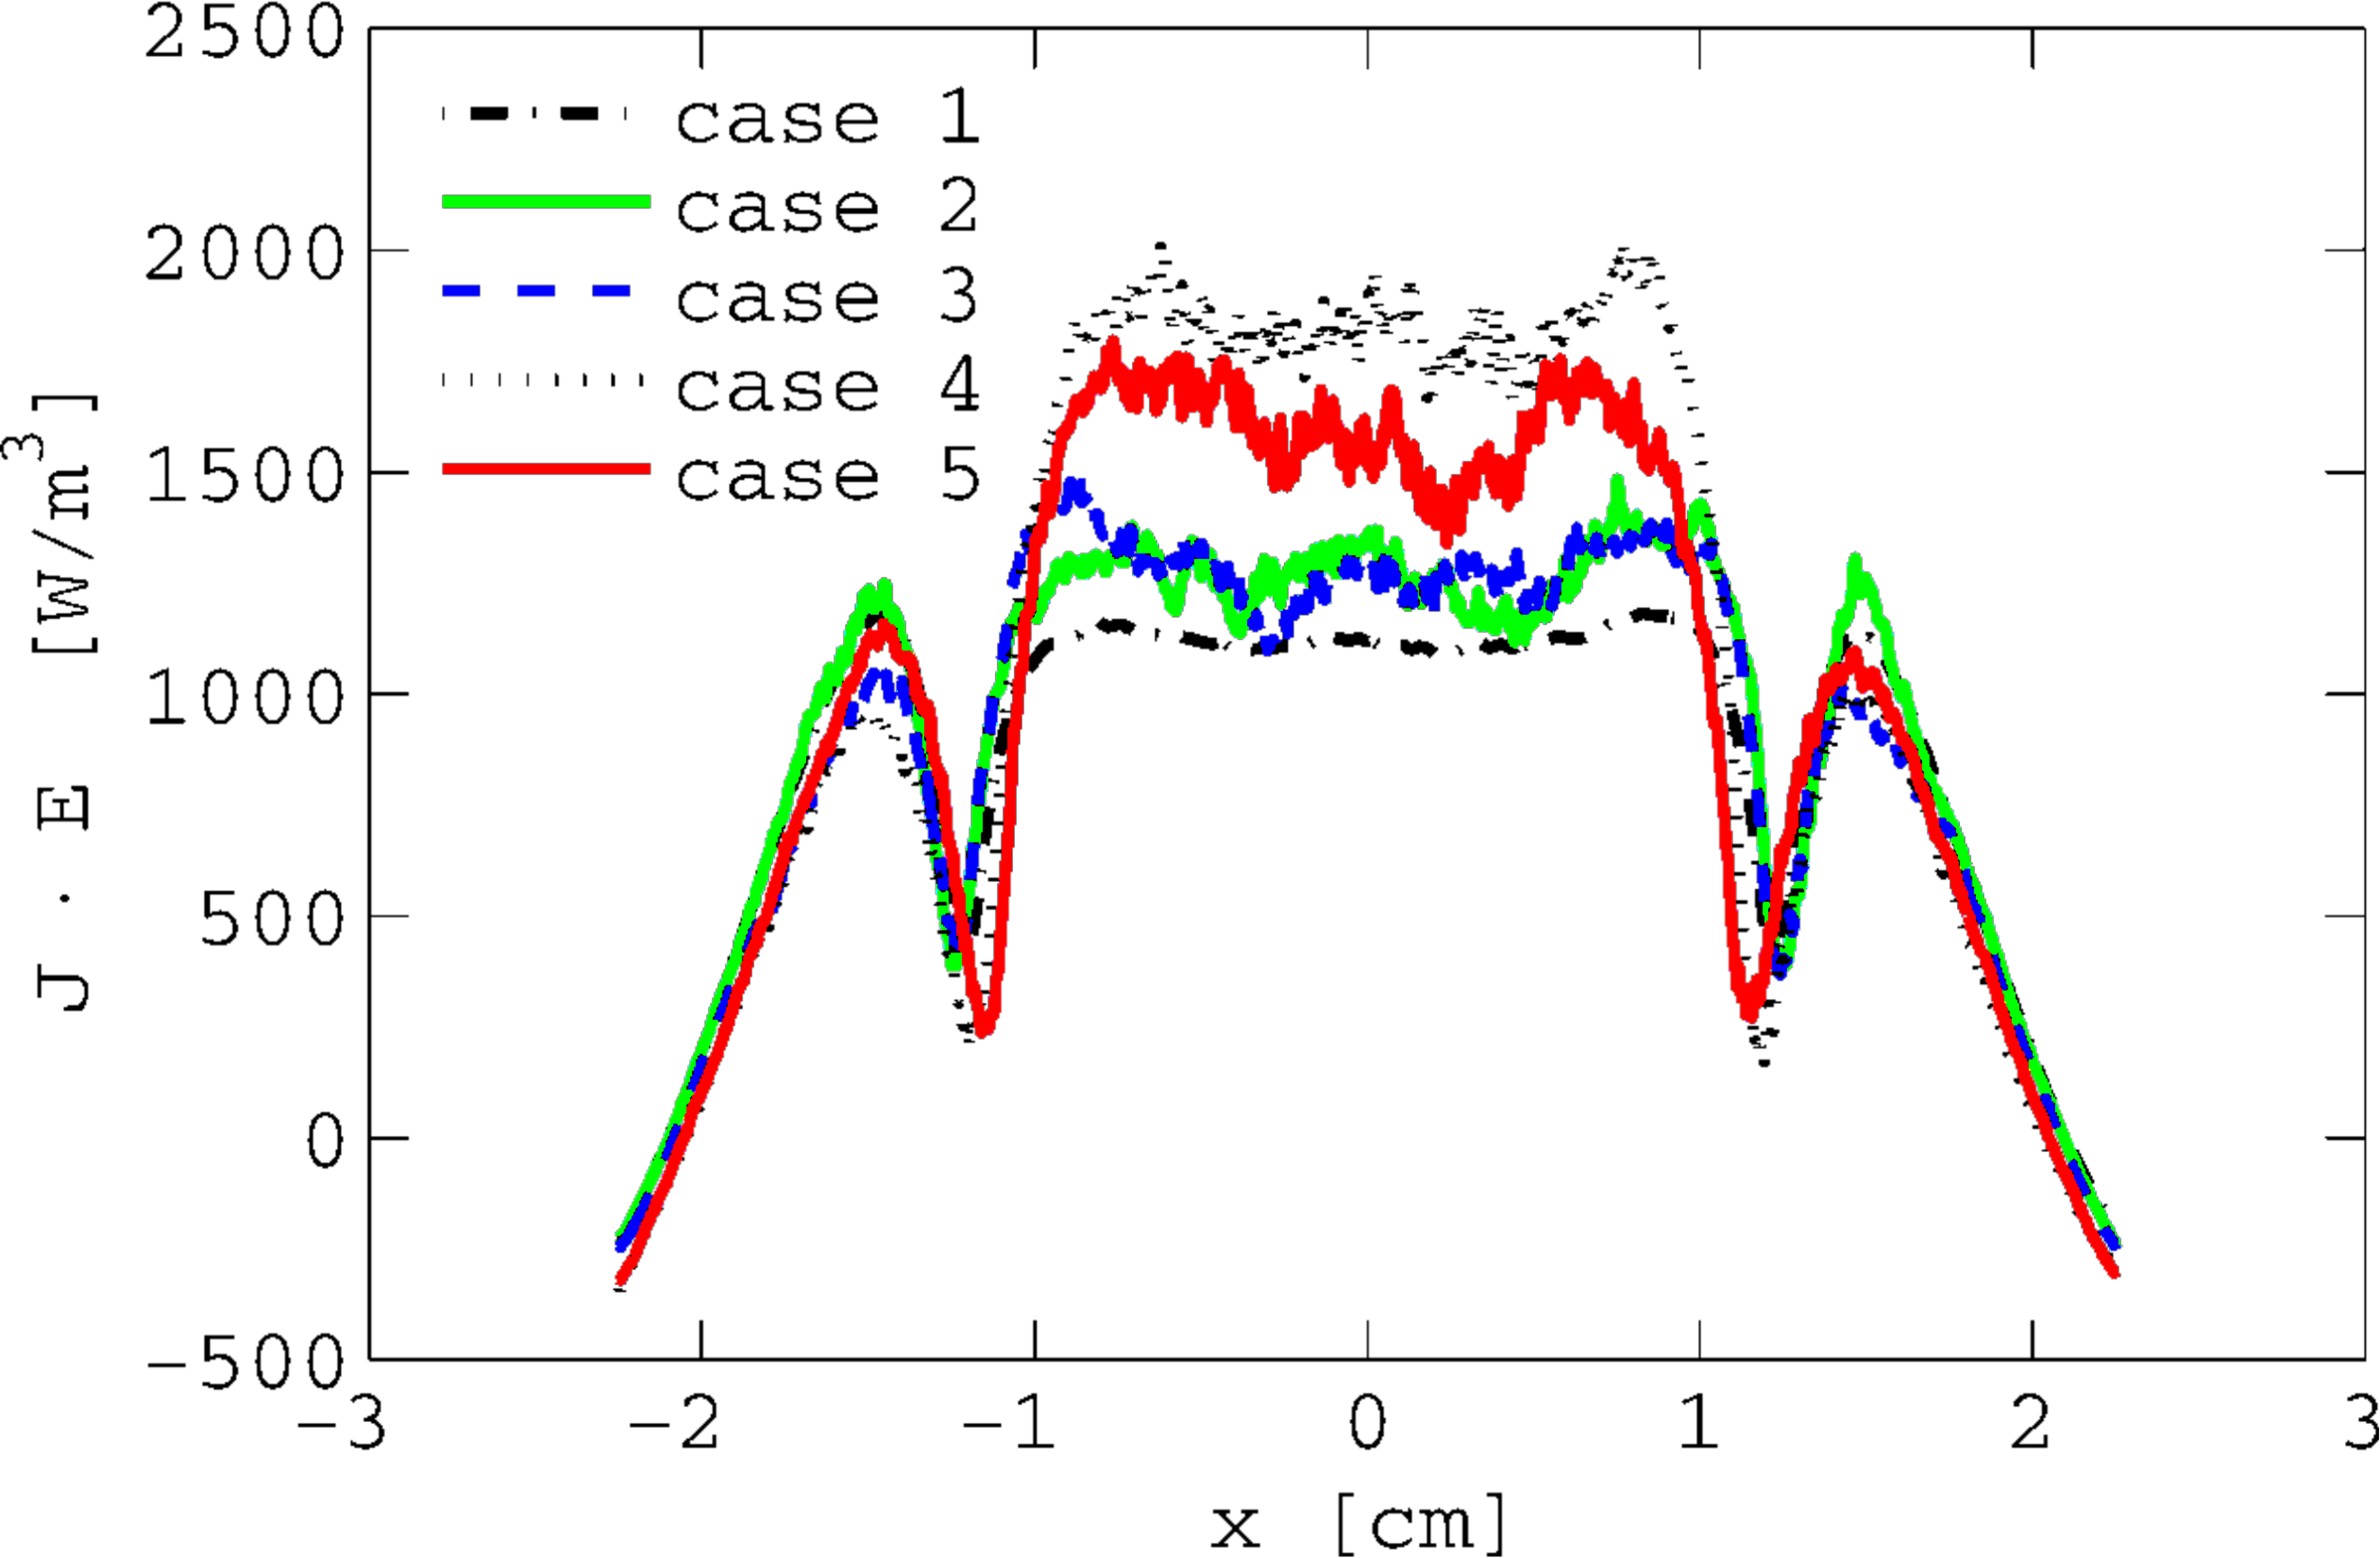
\includegraphics[width=0.7\textwidth]{figures/heatingcomparison.pdf}
			\caption{%
			Electron heating rate for a ccrf discharge of parallel plates at $\unit[6,7]{Pa}$ with an electrode gap of $\unit[4,5]{cm}$ at $\unit[222]{V}$. Other corresponding plasma parameters are noted in~\autoref{tab:comparisonheating}.~\cite{Gudmundsson13}}\label{fig:heatingcomparison}
		\end{figure}
%		
		\begin{figure}[t!]
			\centering
  		\begin{longtable}{lccccr}
				\toprule%
					Case & $\Phi\ix{0}$ & $n\ix{e,0}$/$\unit{m^{-3}}$ %
					& $n\ix{i-,0}$/$\unit{m^{-3}}$ & $n\ix{i+,0}$/$\unit{m^{-3}}$ %
					&	$T\ix{e,0}$/$\unit{eV}$ \\%
		    \toprule\midrule\endhead%
				1 & 101,30 & $2,43\cdot\tenpo{14}$ & $1,17\cdot\tenpo{16}$ %
				& $1,20\cdot\tenpo{16}$ & 2,83 \\ \midrule%
				2 & 101,25 & $2,29\cdot\tenpo{14}$ & $1,21\cdot\tenpo{16}$ %
				& $1,23\cdot\tenpo{16}$ & 2,98 \\ \midrule%
				3 & 101,75 & $2,18\cdot\tenpo{14}$ & $1,19\cdot\tenpo{16}$ %
				& $1,20\cdot\tenpo{16}$ & 2,98 \\ \midrule%
				4 & 103,11 & $1,55\cdot\tenpo{14}$ & $1,75\cdot\tenpo{16}$ %
				& $1,78\cdot\tenpo{16}$ & 3,59 \\ \midrule%
				5 & 102,55 & $1,65\cdot\tenpo{14}$ & $1,70\cdot\tenpo{16}$ %
				& $1,71\cdot\tenpo{16}$ & 3,43 \\ \midrule%
    	\bottomrule%
			\caption{%
				Selected plasma parameters for the used cases in~\autoref{fig:heatingcomparison} at the center of the discharge.~\cite{Gudmundsson13}}\label{tab:comparisonheating}
			\end{longtable}
		\end{figure}
%
		\begin{align}
			\Delta v=v\ix{n+1}-v\ix{n}=-2\,\omega\,%
			s\ix{0}\frac{U\ix{rf}}{U\ix{sb}}\,\sin\varphi\ix{n}%
			\label{equ:deltavheating}
		\end{align}
%	
		A question to answer is what parameter defines the degree of randomization required for an ample stochastical heating in the plasma sheath. Therefore, $K$ is defined as a function of phase-space chaos by eletron energy. Additionally, a simple condition for stochastical motion is derived at the same time.
%
		\begin{align}
			K=\alpha\,\beta\,\frac{U\ix{sb}}{\epsilon E}\,,%
			\quad\quad%
			E\,<\,m\ix{e}\,\omega^{2}s\ix{0}\,l\,\frac{U\ix{rf}}{U\ix{sb}}%
			\label{equ:randomization}
		\end{align}
%
		As is well known~\cite{Goedde88}, chaotic motion occurs in this mapping for $K>1$. It decreases with increasing energy, so the system is less stochastic at higher energies. This is due to the shrinking phase shift across the discharge volume with higher energies. Hence phase corellations between successive collisions in and with the plasma sheath reduce stochasticity.\\
		Last, but not least, one calculates the instantaneous power dissipated into the plasma due to this heating mechanism. Here, using the sheath speed from above $u\ix{s}$, the electron drift velocity $u\ix{e}$ and the maxwellian electron velocity distribution funtion $f\ix{v}(v\ix{e},t)$, Lieberman~\cite{Lieberman88} finds
%
		\begin{align}
			P\ix{stoc}(t)=-2m\ix{e}\int_{u\ix{s}}^{\inf}\,u\ix{s}%
			{\left(v\ix{e}-u\ix{s}\right)}^{2}\,f\ix{v}(v\ix{e},t)\diff v=%
			2\,n\ix{e,0}u\ix{e}k\ix{B}T\ix{e}\sin(\omega t)%
			\label{equ:powerdepositheat}
		\end{align}
%
		Clearly, this results yields not net heating if averaged over one rf cycle. That is, if the current used would be conserved in a manner the HWA is predicting it, or the electron drift velocity does not satisfy the maxwellian distribution function. Hence, there have to be deviations from the proposed theory of stochastical heating. This would be e.g.\@ ab initio information about the EEDF, unconsidered transit time effects of the sheath electric field and neglected particle losses and current conservation.\\
		Therefore more theoretical approaches on the heating in low-pressure, low-temperature rf plasma. For example, Surendra et al~\cite{Surendra93} put forth the idea that the compression and decompression of the electron density volume between opposing plasma sheaths generates heat inside the bulk is responsible for the observed heating.\\
		The electron heating profile is shown in~\autoref{fig:heatingcomparison}. The electron heating peaks near the sheath edges are due to the stochastic heating while the main plateau in the bulk is a result of the dominantly strong ohmic heating with slow electrons and neutral gas friction.
